\chapter{Future Improvements - Vector Boson Fusion HH Production}\label{ch:vbf}
\quoteAuthor{Do not be too timid and squeamish about your actions. All life is an experiment. The more experiments you make the better.}{Ralph Waldo Emerson}

To improve this analysis, a signal model for the Vector Boson Fusion production mode has been designed and will be implemented into this analysis using the full \RunTwo dataset. This signal model is integrated into the analysis through a separate analysis category that is enriched in VBF events, defined via cuts on multiclass \gls{BDT} scores.

This chapter outlines the approach to defining the signal selection for the \gls{VBF} production mode. Section~\ref{sec:vbf-samples} describes the \gls{MC} simulation produced to model VBF \hhyybb production. Section~\ref{ssec:vbf-event-selection} outlines improvements in signal selection for the analysis, starting with a \gls{BDT} used to define analysis categories focused on ggF \hh production (Section~\ref{ssec:ggf-bdt}), followed by a separate multiclass \gls{BDT} used to define a VBF-enriched signal category (Section~\ref{ssec:vbf-bdt}). Adding such a category takes advantage of the unique \gls{VBF} topology to improve the overall Asimov significance, and also provides sensitivity to additional couplings, most notably the $c_{2V}$ coupling corresponding to the interaction between the two vector bosons and two Higgs bosons, which can lead to significant increases in the \hh cross--section, described in Section~\ref{sssec:vbfHH}.

\section{Simulated Samples}\label{sec:vbf-samples}

\subsection{Non-resonant VBF HH Samples}\label{ssec:vbf-samples-production}

The signal MC samples\footnote{Samples with varied coupling strengths were also produced, described in Appendix~\ref{app:vbf-couplings}.} for VBF $HH$ production are generated at LO using \MGMCatNLO 2.6.0, using cards presented in~\cite{vbfhh}. The process generated is $pp \rightarrow HHqq$. The dominant production in this sample is VBF \hh production, but contains contributions from $VHH$ hadronic and Higgsstrahlung production. While these additional production modes are not \gls{VBF} \hh production, they do not overlap with the \gls{ggF} \hh sample, since the generated process differs. The generated \gls{VBF} sample requires $pp$ interactions producing two Higgs bosons and two additional jets, where the \gls{ggF} sample requires the production of two Higgs bosons without additional jets. The \texttt{NNPDF 2.3 LO} PDF set~\cite{NNPDF} is used in the matrix element, interfaced to \HERWIG 7.0.4 using the \texttt{H7-UE-MMHT} tune for underlying events and the \texttt{H7-MMHT2014LO} tune for parton shower and hadronization.

\subsection{Non-resonant ggF HH Samples}

The ggF \hh sample produced in these studies matches the non-resonant \gls{SM} signal sample described in Section~\ref{sssec:signal-samples}, however is produced for the full \RunTwo dataset, with independent samples produced to match running conditions in the 2017 and 2018 data taking periods in addition to the 2015+2016 sample.

\subsection{Background Samples}\label{ssec:vbf-bkg-samples}

The same \yy-continuum processes described in Section~\ref{sssec:background-samples} are the predominant background in these studies. Dominant mono-Higgs backgrounds described in Section~\ref{sssec:background-samples} are considered as well, $ttH$, $ZH$, and $ggH$. Both of these have been produced to match the conditions of the full \RunTwo data taking period.

Additionally, \gls{NTNI} data, which fails photon identification, isolation, or both, is considered to model $\gamma j$, $j \gamma$, and $jj$ contributions. The yield is proportionally scaled to the template fits, described in Section~\ref{ssec:background-composition}. Last, a sample of top-quark pair production associated with 2 photons, $tt \yy$, is used. This sample is produced at \gls{LO} using \MADGRAPH, showered with \peight using the \texttt{A14} tune and the \texttt{NNPDF23LO} PDF set.


\section{Event Selection}\label{ssec:vbf-event-selection}

To improve the event selection presented in Section~\ref{sec:yybb-event-selection} events are evaluated by a \gls{BDT} trained to target \hh production, described in Section~\ref{ssec:ggf-bdt}. Then the \gls{VBF} enriched signal region is constructed, described in Section~\ref{ssec:vbf-bdt}. Events considered have the following preselection cuts are applied:

\begin{itemize}
	\item $N_{\text{cen jets}} < 6$, to help reject $ttH$ production (hadronic top decays).
	\item $N_{\text{lep}} = 0$, to help reject $ttH$ production (leptonic top decays).
	\item $N_{\text{85 \% b-tags}} >= 2$.
	\item $N_{\text{70 \% b-tags}} < 3$, to maintain orthogonality with the $HH \rightarrow \bb\bb$ analysis.
\end{itemize}



\subsection{BDT for ggF Production}\label{ssec:ggf-bdt}
A \gls{BDT} has been trained in order to maximize signal efficiency for ggF \HH production\footnote{This \gls{BDT} has been developed within the full \hhyybb analysis group. While contributions were made to early \gls{ggF} BDTs, the focus of the work presented is on the \gls{VBF} selection. The \gls{ggF} \gls{BDT} is constructed to target di-Higgs production, and is used as a prerequisite for selection into the \gls{VBF} category. Further, the signal categories defined with this \gls{BDT} are used as a benchmark to evaluate improvement in significance, so a description is included.}. Following preselection, events are segmented into two regions, a high mass region with ${m_{X^{*}} > \unit{350}{\GeV}}$ targeting the standard model signal, and a low mass region with ${m_{X^{*}} < \unit{350}{\GeV}}$ targeting \gls{BSM} signals. 

%\footnote{The \glspl{BDT} presented in this chapter use the \texttt{XGBoost} library~\cite{XGBoost}. Data manipulation is performed using the \texttt{Numpy} library~\cite{numpy}}

In each region, a separate BDT is trained using a benchmark \HH signal against a combination of \yy, $ttH$, $ggH$, and $ZH$ backgrounds. In the high mass region, the standard model \HH sample is used as signal, while in the low mass region, the ${\klambda = 6}$ sample is used as signal.

The following inputs are used:

\begin{itemize}
	\item{The $p_{T}/m_{\yy}$, $\eta$, $\phi$ of the two photons.} 
	\item{The $p_{T}$, $\eta$, $\phi$, and pseudo-continuous b-tagging score of the first two jets.}
	\item{The MET and the $\phi$ angle of the MET.}
	\item{The $p_{T}$, $\eta$, $\phi$, and mass of the $H\rightarrow \bb$ candidate.}
	\item{The $H_{T}$ (scalar $p_{T}$ sum of all jets).}
\end{itemize}
where,
\begin{itemize}
	\item{The $p_{T}$ of the two photons are scaled by $m_{\yy}$ to prevent the BDT from learning the $m_{\yy}$ variable. There is no equivalent scaling done for the two jets, since fitting is performed in $m_{\yy}$, not $m_{\bb}$.}
	\item{Jets are ordered by pseudo-continuous b-tagging score, and then by $p_{T}$ in case of a tie. The $H \rightarrow \bb$ candidate is then formed by the two highest ranked jets by simply summing their four-vectors.}
	\item{All vectors are rotated by the same $\phi$ angle so that the $\phi$ of the leading photon is equal to zero. This effectively removes one degree of freedom for the BDT to learn.}
\end{itemize}

After training, two categories are created in each mass region by creating cuts on the BDT output. The category boundaries are optimized to give the best Asimov number counting significance~\cite{asimov}, given by
\begin{equation}\label{eqn:asimov-significance}
    Z = \sqrt{2[(s+b)\log{(1 + s/b)} -s]}.
\end{equation}
The signal, $s$, is the sum of both ggF and VBF \hh contributions in a category. The background, $b$, is the sum of the considered backgrounds described in Section~\ref{ssec:vbf-bkg-samples}: \yy-continuum processes, \gls{NTNI} data to model jets faking photons, leading mono-Higgs production modes ($ttH$, $ZH$, and $ggH$), and $tt\gamma\gamma$. The four signal categories (two mass regions, each with two categories) are added in quadrature for the final Asimov significance of 0.415 using the full 140 \ifb collected in \RunTwo.


\subsection{BDT for VBF Production}\label{ssec:vbf-bdt}
On top of the ggF \gls{BDT} selection, a dedicated VBF-enriched analysis category is built. Events which have already passed the ggF BDT based selection and have at least four jets are considered the VBF category. The four jet requirement is imposed in order to reconstruct VBF-based variables, since two jets are needed for the \Hbb decay, and another two are needed for the VBF jets. The VBF jets are then selected as the highest $m_{jj}$ pairing, excluding $H\rightarrow b\bar{b}$ candidate jets.

These events are then evaluated by a multiclass BDT, which has independent classes for VBF \HH, ggF \HH, \yy-continuum, and $ttH$. This model was chosen due to large $ttH$ contamination in the VBF enriched category by binary classifiers considering just \yy-continuum backgrounds. Ultimately, an event selected for the VBF category if it passes the BDT score threshold for VBF \HH, and fails the score threshold for the other three classes. A flowchart of this logic is shown in Figure~\ref{fig:vbf-logic}.

\begin{figure}[htbp]
    \centering
	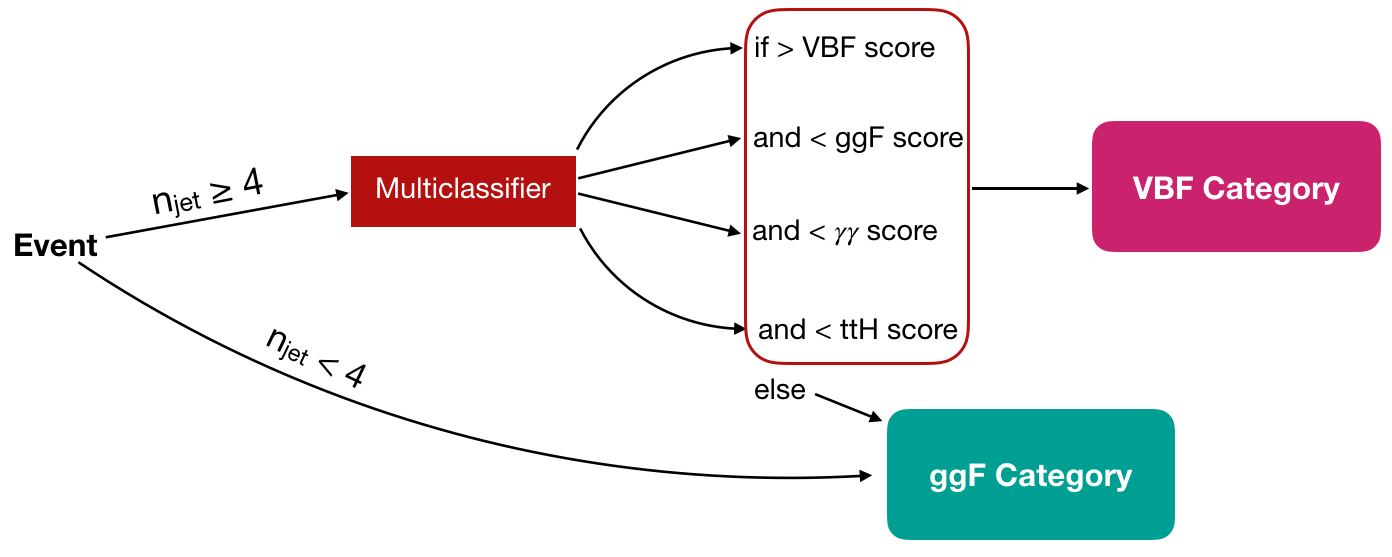
\includegraphics[width=0.9\textwidth]{chapters/chapter6_vbf/images/vbf_logic.png}
    \caption[Logic flow for an event to be selected into the VBF-enriched signal region]{Logic flow for an event to be selected into the VBF-enriched signal region. The starting set of candidates (denoted ``event'') requires passing preselection and at least one of the ggF-based signal categories. If an event is assigned to the ggF categories, it is separated into 4 categories by the \gls{BDT} described in Section~\ref{ssec:ggf-bdt}.}
    \label{fig:vbf-logic}
\end{figure}

\subsubsection{Input Selection}
A set of 26 variables were considered for this BDT, listed in Appendix~\ref{app:vbf-variables}. Broadly, they describe the kinematics of various physics objects in the event, as well as event shape variables~\cite{STDM-2011-33} and variables to reconstruct the $W$ and top mass, which aim to suppress the $ttH$ background.

For dimensionality reduction, a pruning procedure was performed.
\begin{enumerate}
  \item To remove redundant variables, those with a Pearson correlation value above 0.85 were removed. This brought the list from 26 to 19, pruning several event shape variables.
  \item After pruning those variables and retraining, low-impact variables were removed. The Pearson correlation for each variable to the 4 class \gls{BDT} probability distributions were calculated. Those 4 correlation values were summed, and variables with a sum less than 1.0 were pruned. This brought the set from 19 to 10 input variables.
\end{enumerate}

After this pruning procedure, the 10 final inputs were: 
\begin{itemize}
\item \textbf{VBF-targeted:} $\Delta \eta_{jj}$, $m_{jj}$.

\item \textbf{$\gamma \gamma$-suppressing:} \myybb, $\Delta R_{\gamma\gamma}$, $\Delta R_{\bb}$, the best b-tagging WP for the $H\rightarrow \bb$ jets.

\item \textbf{$ttH$-suppressing:} Transverse Sphericity ($S_{\perp}$), Planar Flow ($Pf$), $\pt^\text{balance}$.
\end{itemize}
%
$S_{\perp}$ is given in Reference~\cite{STDM-2011-33}, Planar Flow is given in Reference~\cite{planar-flow}, and $\pt^\text{balance}$ is given by:

\begin{equation}\label{eqn:pt-balance}
    \pt^\text{balance} = \frac
    {| \vec{p}_T^{\gamma_1} + \vec{p}_T^{\gamma_2} + \vec{p}_T^{j_1} +  \vec{p}_T^{j_2}|}
    {|\vec{p}_T^{\gamma_1}| + |\vec{p}_T^{\gamma_2}| + |\vec{p}_T^{j_1}| +  |\vec{p}_T^{j_2}|}.
\end{equation}
%
Distributions for each these variables after applying a 4-jet requirement can be found in Appendix~\ref{app:vbf-variables}. 

\subsubsection{Model Optimization}

This section outlines two optimizations performed in the definition of the VBF-enriched category. First, the optimization of the model's main hyperparameters. Second, the selection of cuts on the \gls{BDT} scores to define the \gls{VBF} signal category. For these optimizations, an orthogonal sample of events must be selected to ensure the model is generalizable. A subset of 50\% of the data is used for training, 25\% for testing, and 25\% for model selection\footnote{This split is done using the ATLAS global event number. A modulo 4 operation is performed on the event number, if the result is 0 or 1, it is used in the training sample. If the result is 2, it is used in the testing sample. If the result is 3, it is used in the model selection sample.}.

\noindent\textbf{Hyperparameter Optimization}\\
\indent The maximum \gls{BDT} depth is selected by training models at increasing depth and selecting the depth when the accuracy on the testing set ceases to improve, a depth of 14. After that point, the accuracy on the training set flattens, while it continues to increase on the testing set, leading to overtraining. The same procedure is performed for the number of trees, evaluating 10, 25, 50, 75, 100, 150, 200, and 300 trees. This parameter flattens for both training and testing, so a safe choice of 200 trees is used. The accuracy as a function of these parameters is shown in Figure~\ref{fig:hp-opt}.

%\footnote{Plots in this chapter are created using the \texttt{Matplotlib} python library~\cite{matplotlib}}

\begin{figure}[!h]
  \centering
  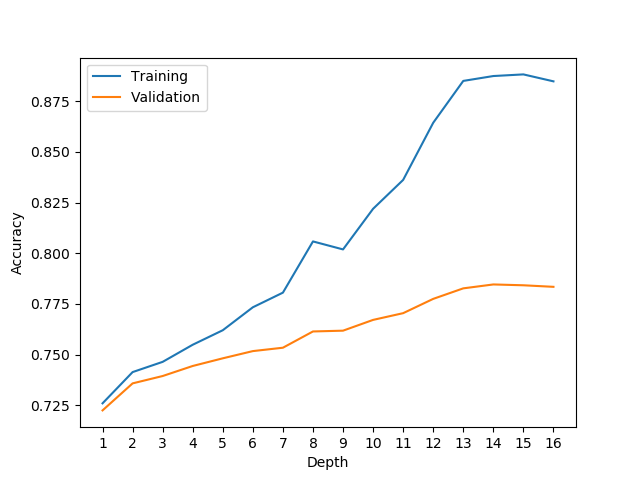
\includegraphics[width=0.48\textwidth]{chapters/chapter6_vbf/images/hp_opt/multiclass_optimized_depth.png}
  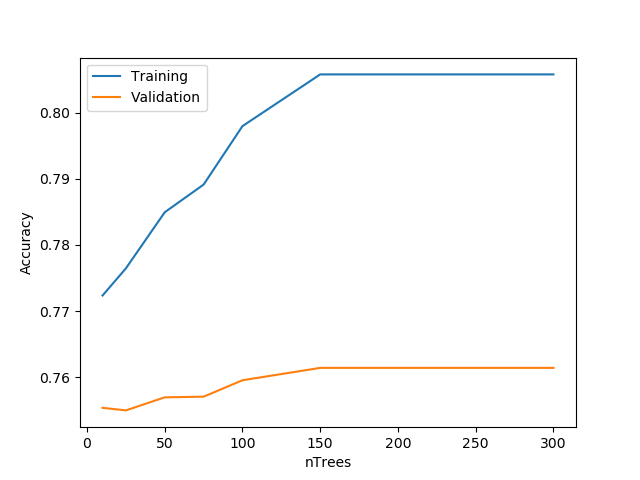
\includegraphics[width=0.48\textwidth]{chapters/chapter6_vbf/images/hp_opt/multiclass_optimized_trees.png}
  \caption[The \gls{BDT} accuracy as a function of hyperparameter values]{The \gls{BDT} accuracy as a function of hyperparameter values. The left is the maximum tree depth, which is chosen to be 14. The right shows the number of trees, which is chosen to be 200. The ``validation'' set is the events used for testing, and orthogonal to the training set.}
  \label{fig:hp-opt}
\end{figure}

\noindent\textbf{BDT Score Cuts}\\
\indent Evaluating an event on this multiclass \gls{BDT} outputs four probabilities, one for each class. These are denoted $p_{\text{class}}$ for each target class, e.g. $p_{\text{VBF}}$ for the class targeting \gls{VBF} \HH production. In order to set the thresholds for each of these probabilities, an optimization procedure is performed. A 4-dimensional scan over the probability scores is performed, in steps of 0.03. At each step, the Asimov significance, given in Equation~\ref{eqn:asimov-significance}, is calculated for each category and summed in quadrature. The contributions to the signal and background components of this equation match that used to evaluate the Asimov significance in Section~\ref{ssec:ggf-bdt}.

Through this optimization procedure, the thresholds shown in Table~\ref{tab:multiclass-thresholds} are found. The output probability distributions for each class on each sample is shown in Figure~\ref{fig:bdt-scores}, with the optimized thresholds overlaid.

\begin{table}[!htb]
  \centering
  \caption[The optimized thresholds for each \gls{BDT} score used to define the VBF-enriched category]{The optimized thresholds for each \gls{BDT} score used to define the VBF-enriched category. The cut threshold of 0.00 on the VBF \hh class means that this class is not cut on.}
  \begin{tabular}{c|c|c}
    \hline
    Class & Target & Selection Logic \\
    \hline
    0 & VBF \HH & $p_{\text{VBF}} > 0.00 $ \\
    1 & ggF \HH & $p_{\text{ggF}} < 0.72 $ \\
    2 & $\gamma\gamma$-Continuum & $p_{\gamma\gamma} < 0.06$ \\
    3 & $ttH$ & $p_{ttH} < 0.81$ \\
    \hline
  \end{tabular}
  \label{tab:multiclass-thresholds}
\end{table}

\begin{figure}[!h]
  \centering
  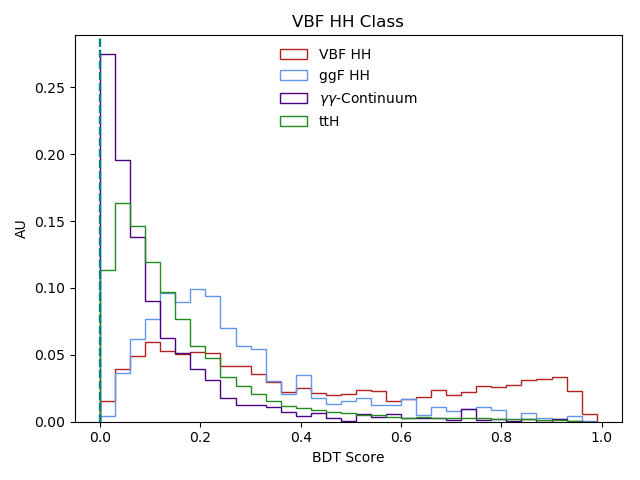
\includegraphics[width=0.48\textwidth]{chapters/chapter6_vbf/images/bdt_scores/vbf_scores.png}
  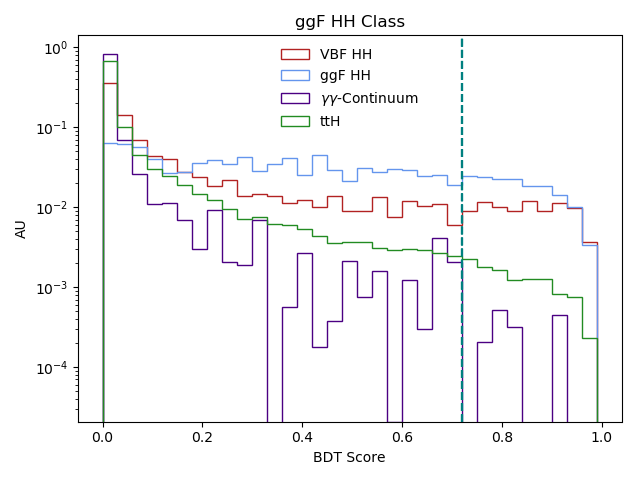
\includegraphics[width=0.48\textwidth]{chapters/chapter6_vbf/images/bdt_scores/log_ggf_scores.png}
  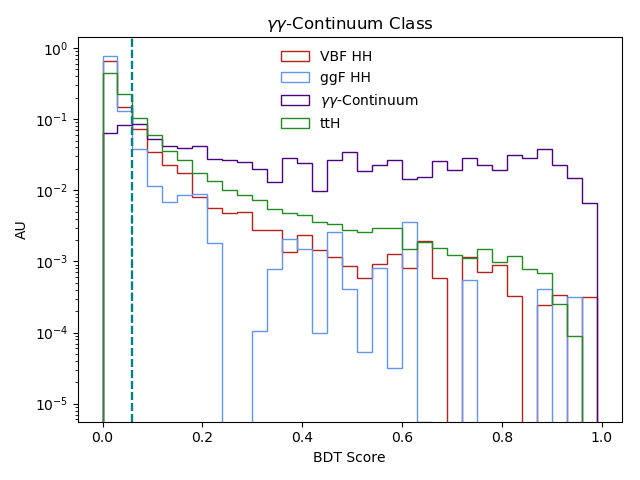
\includegraphics[width=0.48\textwidth]{chapters/chapter6_vbf/images/bdt_scores/log_yy_scores.png}
  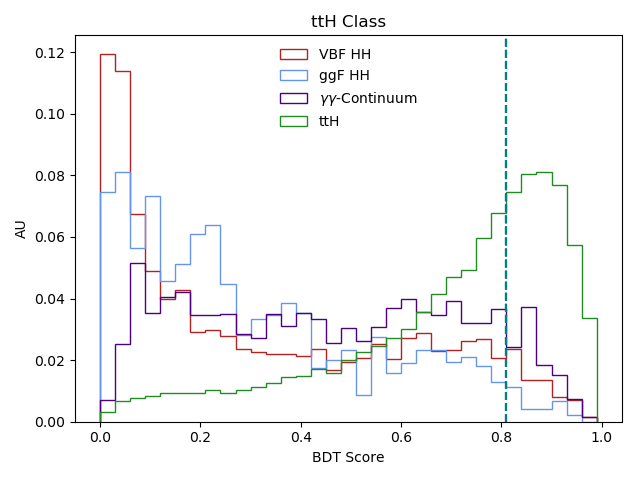
\includegraphics[width=0.48\textwidth]{chapters/chapter6_vbf/images/bdt_scores/tth_scores.png}
  \caption[The \gls{BDT} score distribution for each class, evaluated on the VBF \HH, ggF \HH, \yy-continuum, and $ttH$ samples]{The \gls{BDT} score distribution for each class, evaluated on the testing VBF \HH, ggF \HH, \yy-continuum, and $ttH$ samples. The ggF \HH and \yy-continuum distributions are shown on a log scale. A vertical line showing the cut threshold is shown on each distribution.}
  \label{fig:bdt-scores}
\end{figure}

The contribution of each signal and background process to each category is shown in Figure~\ref{fig:category-yields}. The categorization for each signal process as well as the dominant \yy-continuum background is shown in Figure~\ref{fig:process-categorization}. The \gls{VBF} \hh category is dominated by \gls{ggF} production due to the large difference in cross-sections, however the \gls{VBF} \hh sample is predominantly classified into the \gls{VBF}-targeted signal region. Adding these five categories in quadrature gives an Asimov significance of 0.459, a 9.7\% improvement over not defining such a category.
% The categorization for the mono-Higgs, \gls{NTNI}, and $tt\yy$ samples are shown in Appendix TODO.

\begin{figure}[p!]
  \centering
  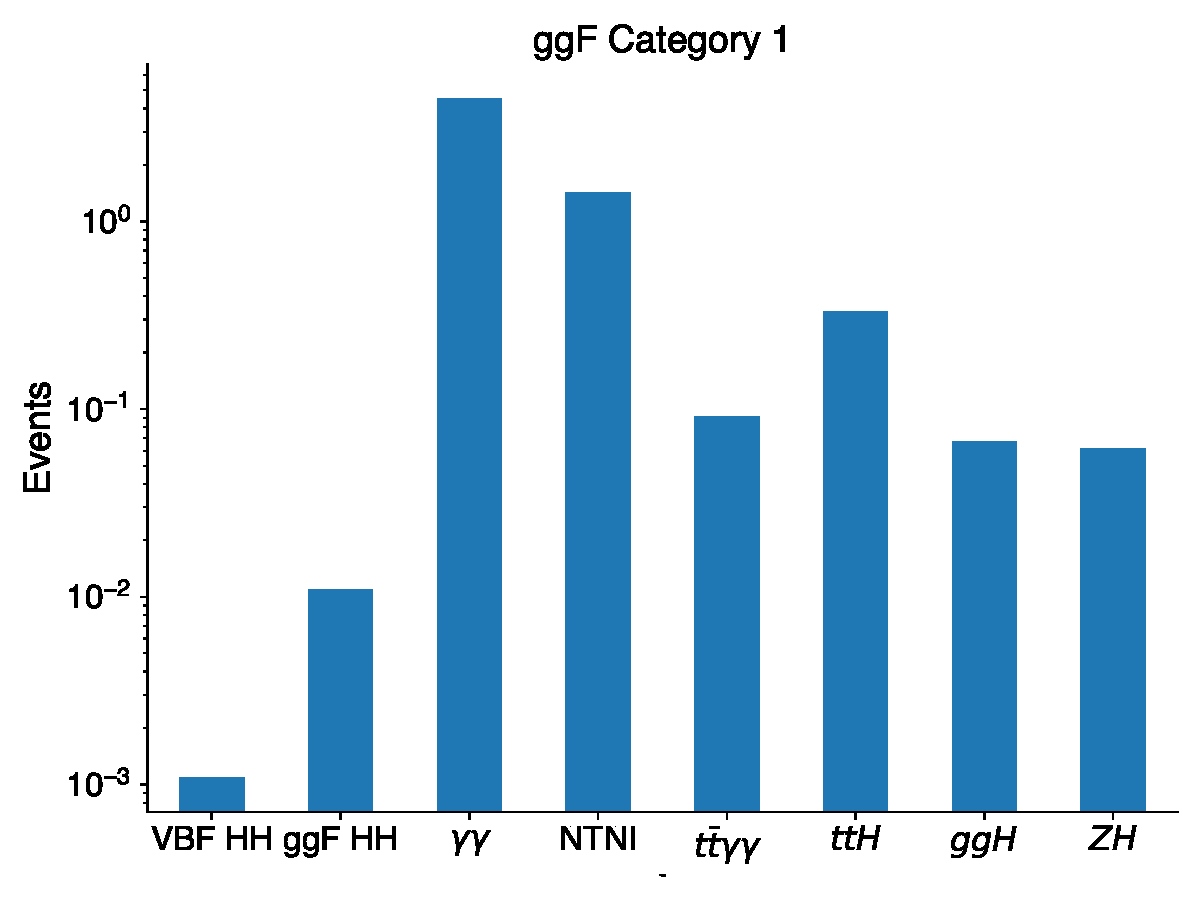
\includegraphics[width=0.48\textwidth]{chapters/chapter6_vbf/images/category_breakdown/ggfcat1.pdf}
  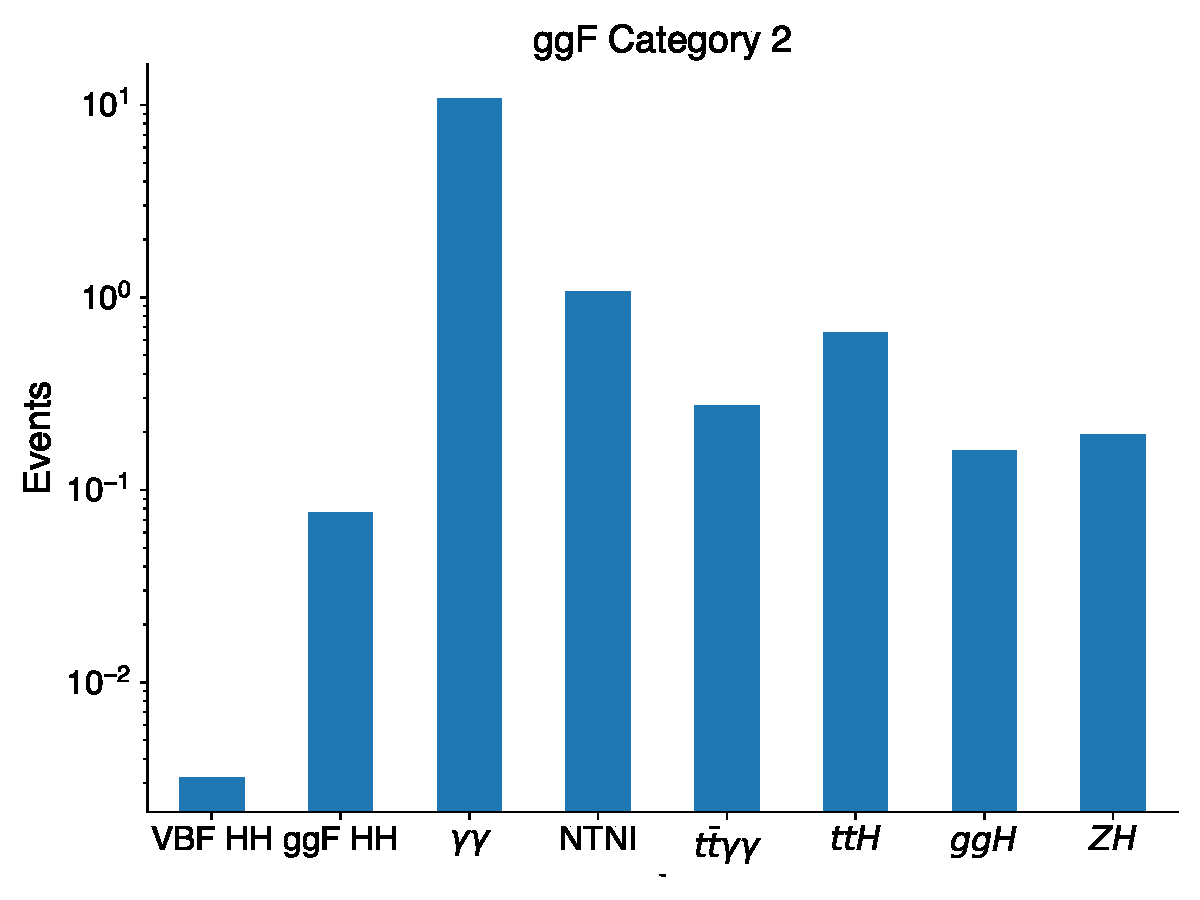
\includegraphics[width=0.48\textwidth]{chapters/chapter6_vbf/images/category_breakdown/ggfcat2.pdf}
  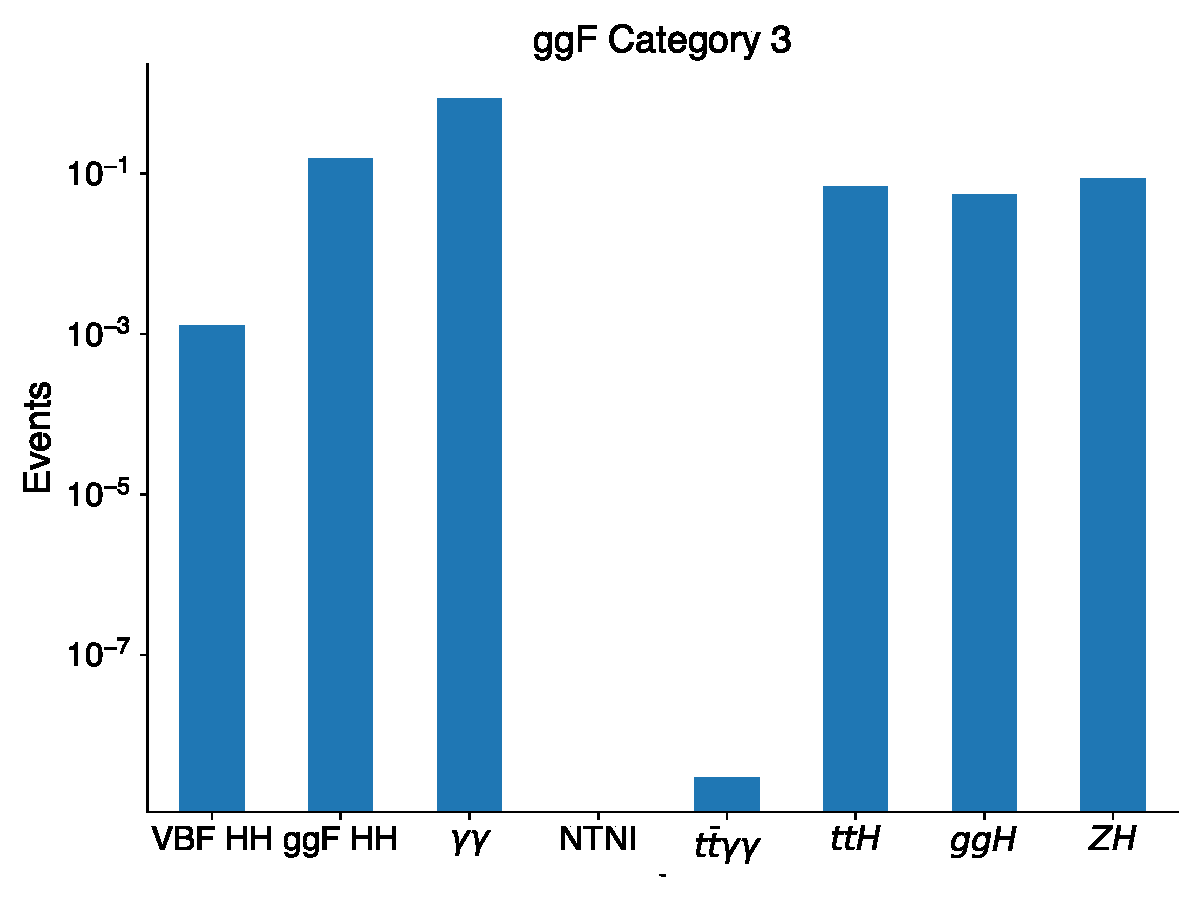
\includegraphics[width=0.48\textwidth]{chapters/chapter6_vbf/images/category_breakdown/ggfcat3.pdf}
  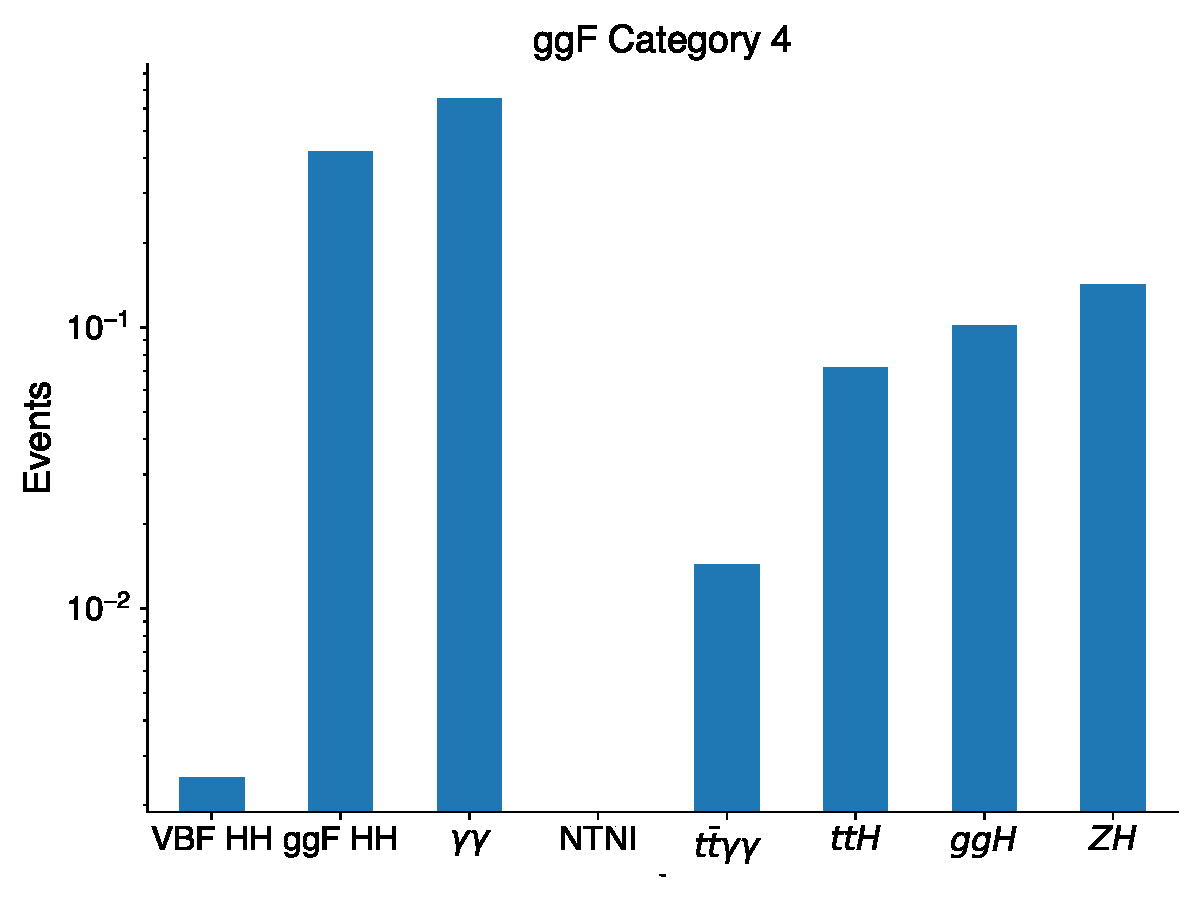
\includegraphics[width=0.48\textwidth]{chapters/chapter6_vbf/images/category_breakdown/ggfcat4.pdf}
  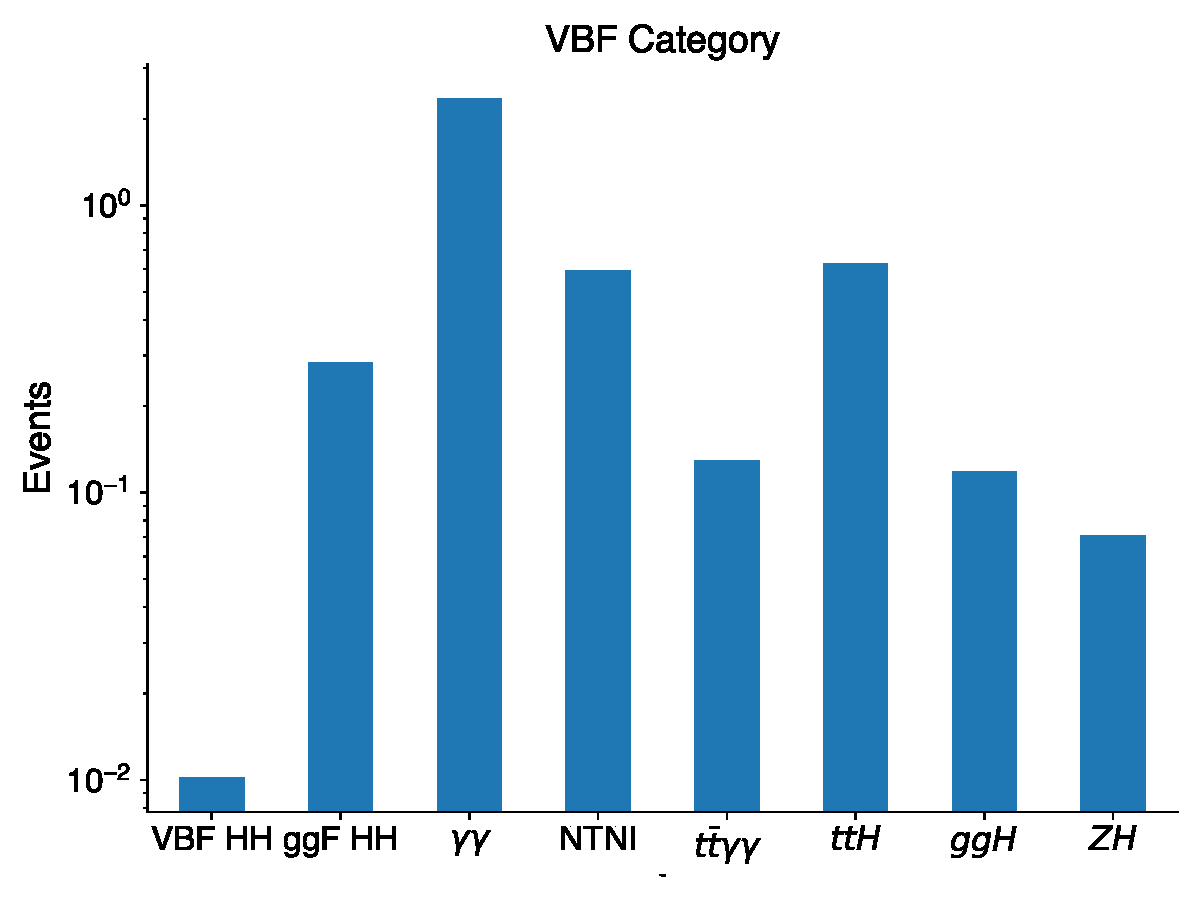
\includegraphics[width=0.48\textwidth]{chapters/chapter6_vbf/images/category_breakdown/vbfcat.pdf}
  \caption[The contribution of signal and leading background samples to each analysis category after adding the optimized VBF-enriched category]{The contribution of signal and leading background samples to each analysis category after adding the optimized VBF-enriched category. VBF and ggF \HH are the two signal production modes considered. $\gamma \gamma$ is the diphoton continuum background, $t\bar{t}\gamma\gamma$ is top-quark pair production associated with 2 photons, and NTNI is not-tight not-isolated data (scaled using a template fit). The three dominant mono-Higgs backgrounds, $ttH$, $ggH$, and $ZH$ are shown. The \gls{ggF} categories correspond to (1) $m_{X^{*}} < \unit{350}{\GeV}$, loose b-tag (2) $m_{X^{*}} < \unit{350}{\GeV}$, tight b-tag (3) $m_{X^{*}} \geq \unit{350}{\GeV}$, loose b-tag (4) $m_{X^{*}} \geq \unit{350}{\GeV}$, tight b-tag.}
  \label{fig:category-yields}
\end{figure}


\begin{figure}
  \centering
  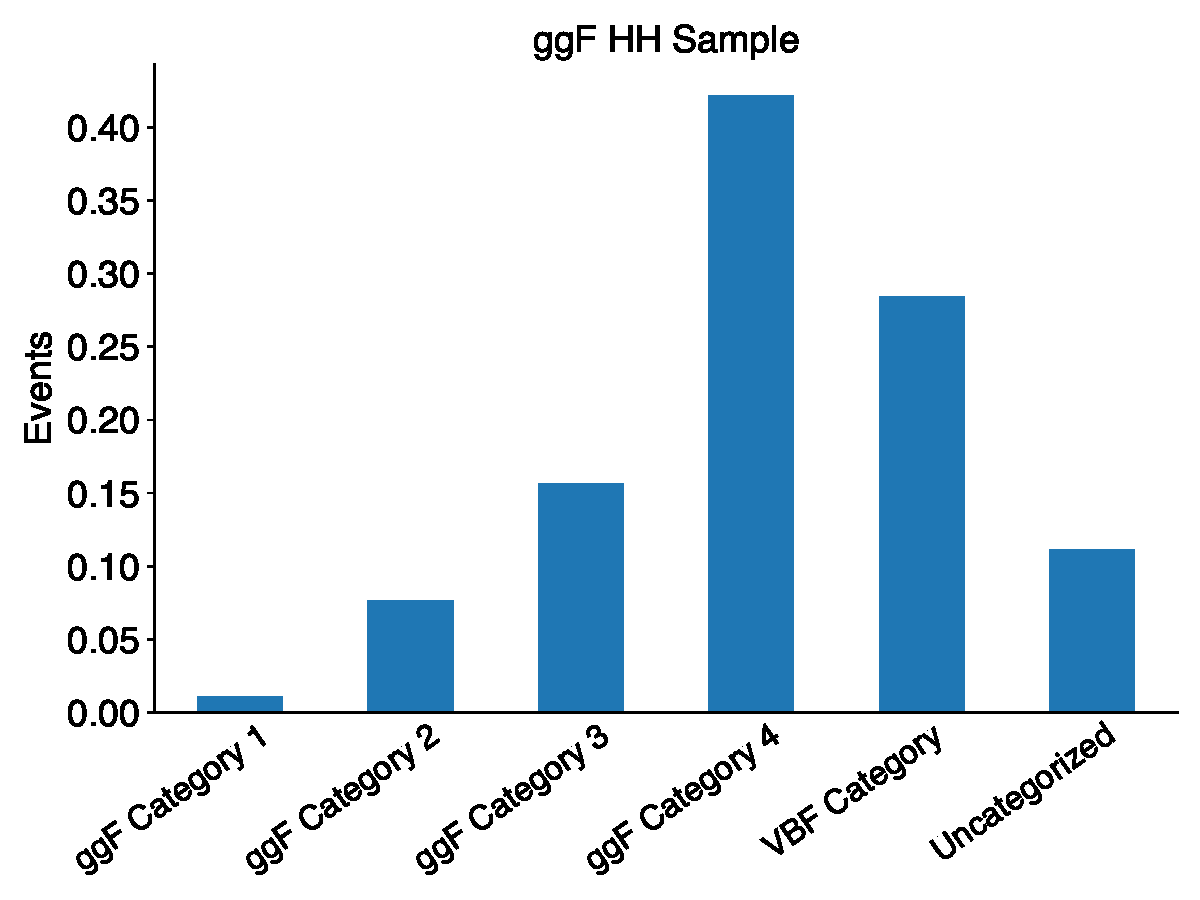
\includegraphics[width=0.48\textwidth]{chapters/chapter6_vbf/images/category_breakdown/ggf_sample.pdf}
  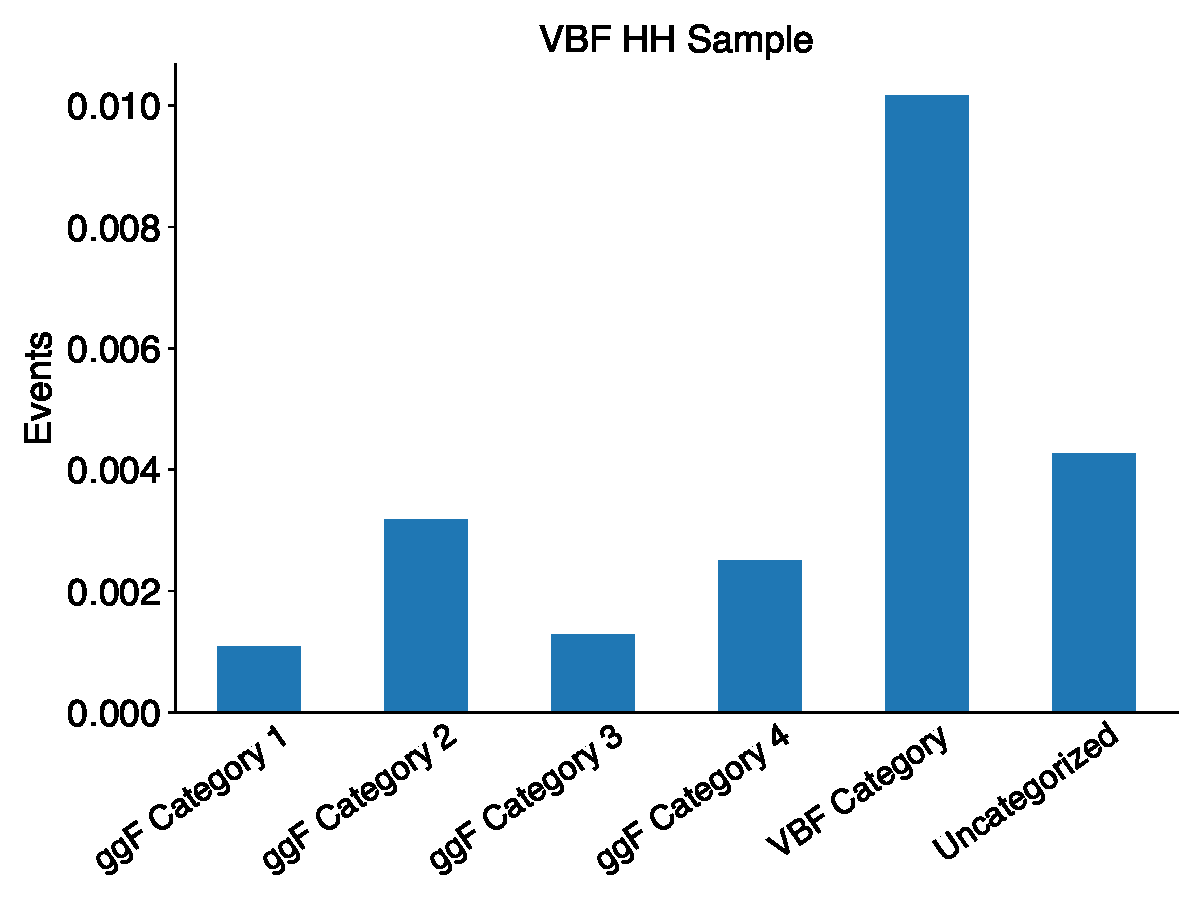
\includegraphics[width=0.48\textwidth]{chapters/chapter6_vbf/images/category_breakdown/vbf_sample.pdf}
  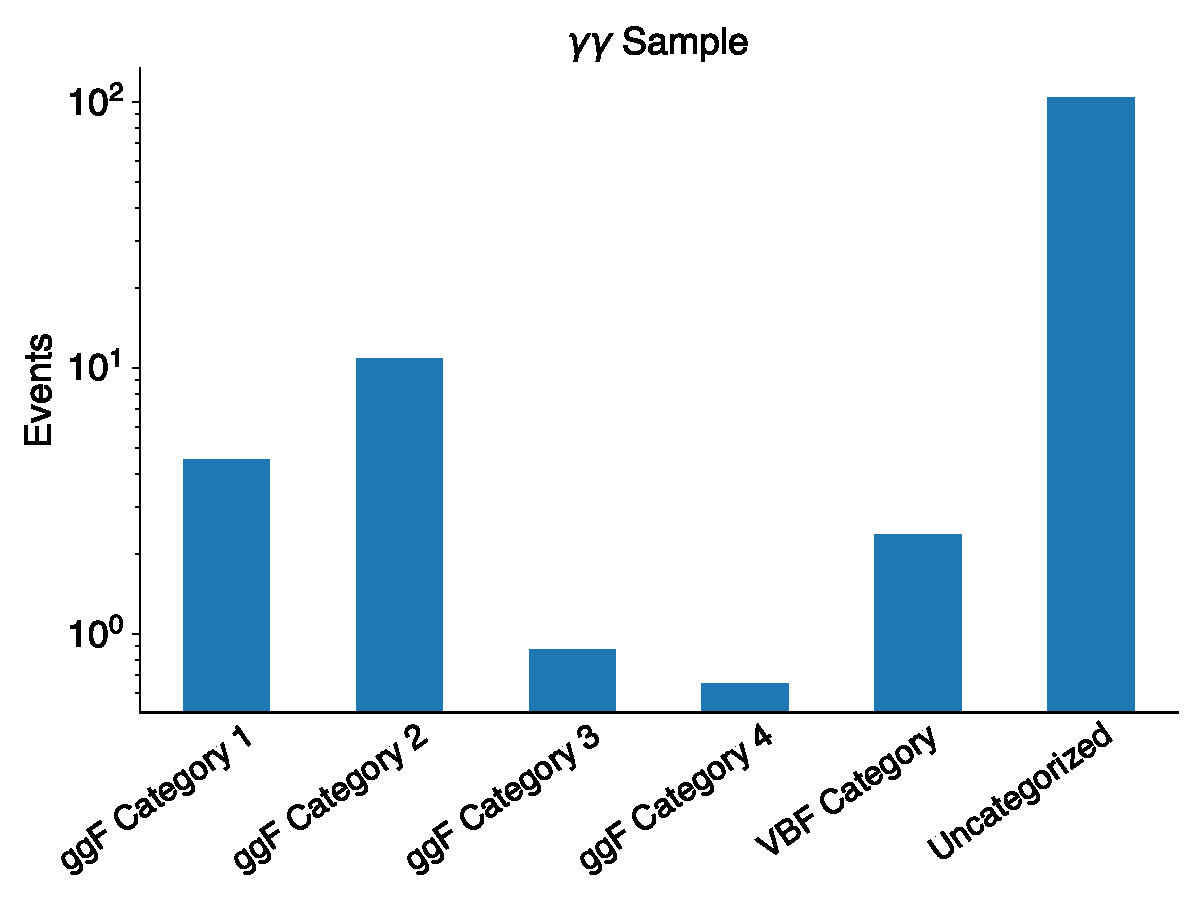
\includegraphics[width=0.48\textwidth]{chapters/chapter6_vbf/images/category_breakdown/yy_sample.pdf}
  \caption[The categorization of the VBF \HH, ggF \HH, and \yy-continuum samples]{The categorization of the VBF \HH, ggF \HH, and \yy-continuum samples. The ``Uncategorized'' bin are events which do not fall into any of the analysis categories. The \yy-continuum plot is shown with log-scale. The \gls{ggF} categories correspond to (1) $m_{X^{*}} < \unit{350}{\GeV}$, loose b-tag (2) $m_{X^{*}} < \unit{350}{\GeV}$, tight b-tag (3) $m_{X^{*}} \geq \unit{350}{\GeV}$, loose b-tag (4) $m_{X^{*}} \geq \unit{350}{\GeV}$, tight b-tag.
  \label{fig:process-categorization}}
\end{figure}



